\documentclass{beamer}
\title{Algorithmic Methods for Mathematical Models\\
 Course Project}
\author{Marco Bartoli, Ilan Vezmarovic}
\institute{UPC Universitat Politècnica de Catalunya}
\date{\today}

\begin{document}

\frame{\titlepage}

\begin{frame}
\frametitle{Formal Problem Definition}
\begin{itemize}
    \item $n$: number of products
    \item $x$: height of the suitcase in millimeters
    \item $y$: width of the suitcase in millimeters
    \item $c$: limit to the total weight of the suitcase in grams
    \item $p_i$: price of the $i$-th product in euros
    \item $w_i$: weight of the $i$-th product in grams
    \item $s_i$: side length of the $i$-th product's (square) box in millimeters
\end{itemize}
\end{frame}


\begin{frame}
\frametitle{Decision Variables}
\begin{itemize}
    \item $\text{Chosen}_i$: binary variable that is 1 if object $i$ is chosen, and 0 otherwise.
    \item $\text{PointsX}_i$: the x-coordinate of the bottom-left corner of object $i$.
    \item $\text{PointsY}_i$: the y-coordinate of the bottom-left corner of object $i$.
    \item $\text{Overlap}_{i,j,d}$: binary variable indicating if objects $i$ and $j$ do not overlap in direction $d$, where $d \in \{1, 2, 3, 4\}$.
\end{itemize}
\end{frame}

\begin{frame}
\frametitle{Objective Function}
Maximize the total price of the chosen objects:

\[
\text{maximize} \sum_{i=1}^n p_i \cdot \text{Chosen}_i
\]
\end{frame}


\begin{frame}
\frametitle{Max Weight Constraint}
Ensure the total weight of the chosen objects does not exceed the suitcase's capacity:

\[
\sum_{i=1}^n w_i \cdot \text{Chosen}_i \leq c
\]
\end{frame}

\begin{frame}
\frametitle{Coordinate Bounds Constraints}
Ensure each object lies entirely within the suitcase's boundaries:

\[
\forall i \in \{1, \ldots, n\}, \quad \text{PointsX}_i \geq 1
\]

\[
\forall i \in \{1, \ldots, n\}, \quad \text{PointsY}_i \geq 1
\]

\[
\forall i \in \{1, \ldots, n\}, \quad \text{PointsX}_i + s_i - 1 \leq x
\]

\[
\forall i \in \{1, \ldots, n\}, \quad \text{PointsY}_i + s_i - 1 \leq y
\]
\end{frame}


\begin{frame}
\frametitle{Non-Overlapping Constraints}
Left/Right/Up/Down non-overlapping:


\[
\forall i, j \in \{1, \ldots, n\}, i \neq j, \quad \text{PointsX}_i - \text{PointsX}_j + s_i \leq
\]
\[
-M \cdot (\text{Chosen}_i + \text{Chosen}_j + \text{Overlap}_{i,j,1} - 3)
\]

\[
\forall i, j \in \{1, \ldots, n\}, i \neq j, \quad \text{PointsX}_i - \text{PointsX}_j + s_i \leq
\]
\[
-M \cdot (\text{Chosen}_i + \text{Chosen}_j + \text{Overlap}_{i,j,2} - 3)
\]

\[
\forall i, j \in \{1, \ldots, n\}, i \neq j, \quad \text{PointsX}_i - \text{PointsX}_j + s_i \leq
\]
\[
-M \cdot (\text{Chosen}_i + \text{Chosen}_j + \text{Overlap}_{i,j,3} - 3)
\]

\[
\forall i, j \in \{1, \ldots, n\}, i \neq j, \quad \text{PointsX}_i - \text{PointsX}_j + s_i \leq
\]
\[
-M \cdot (\text{Chosen}_i + \text{Chosen}_j + \text{Overlap}_{i,j,4} - 3)
\]
\end{frame}

\begin{frame}{Non-Overlapping Constraints}
At least one of the non-overlapping conditions is satisfied:

\[
\forall i, j \in \{1, \ldots, n\}, i \neq j, \quad \sum_{d=1}^4 \text{Overlap}_{i,j,d} \geq 1
\]
    
\end{frame}

\begin{frame}
\frametitle{Time chart}
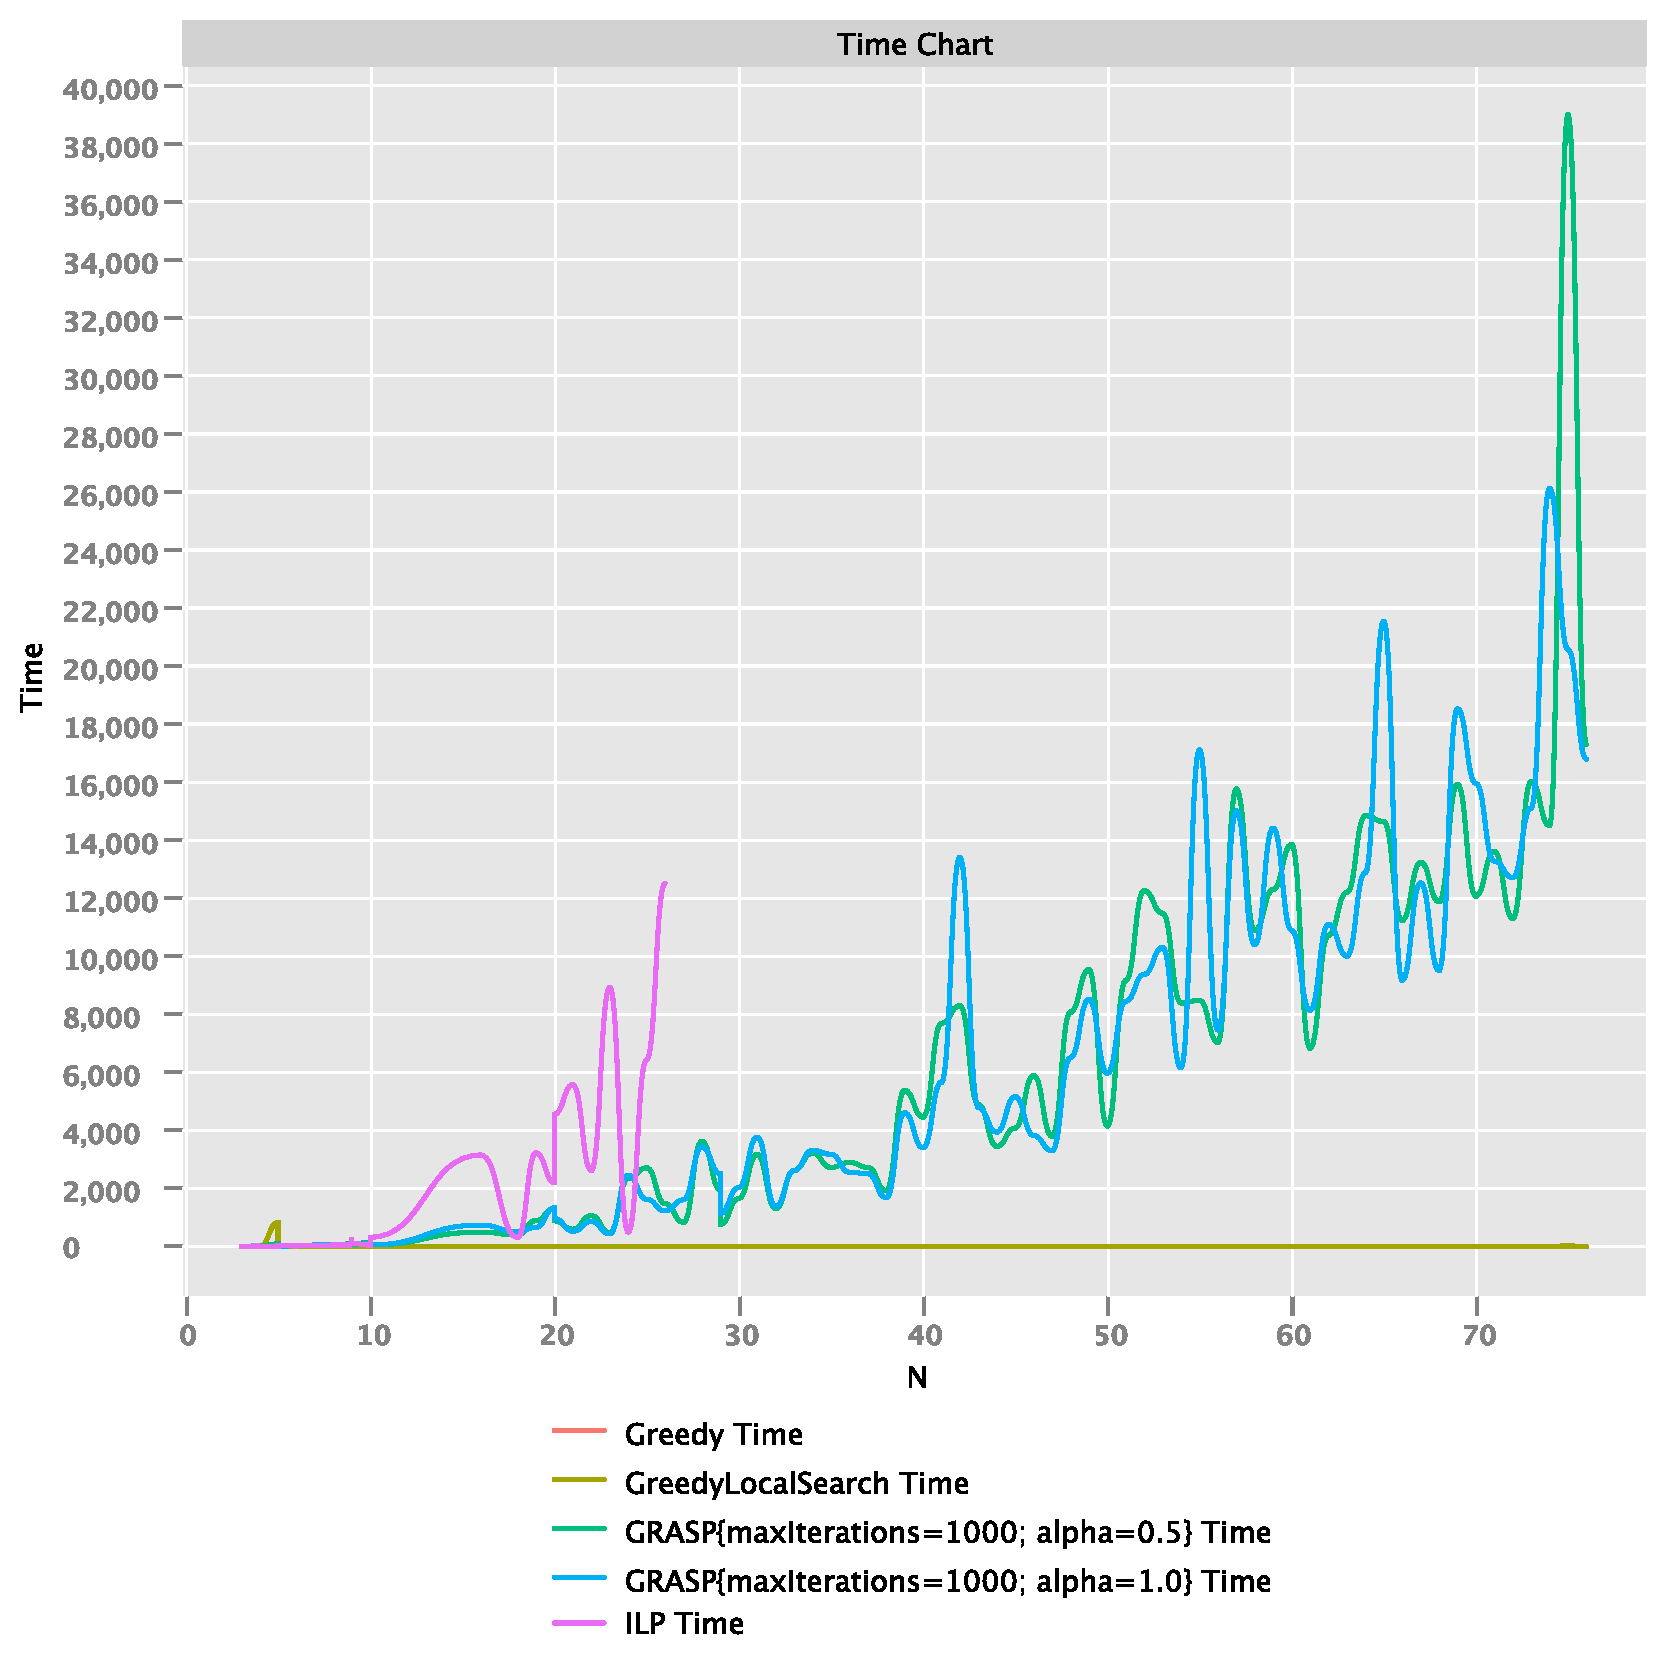
\includegraphics[width=0.8\textwidth]{./documentation/assets/timeChart.pdf}
\end{frame}

\begin{frame}
\frametitle{Objective chart}
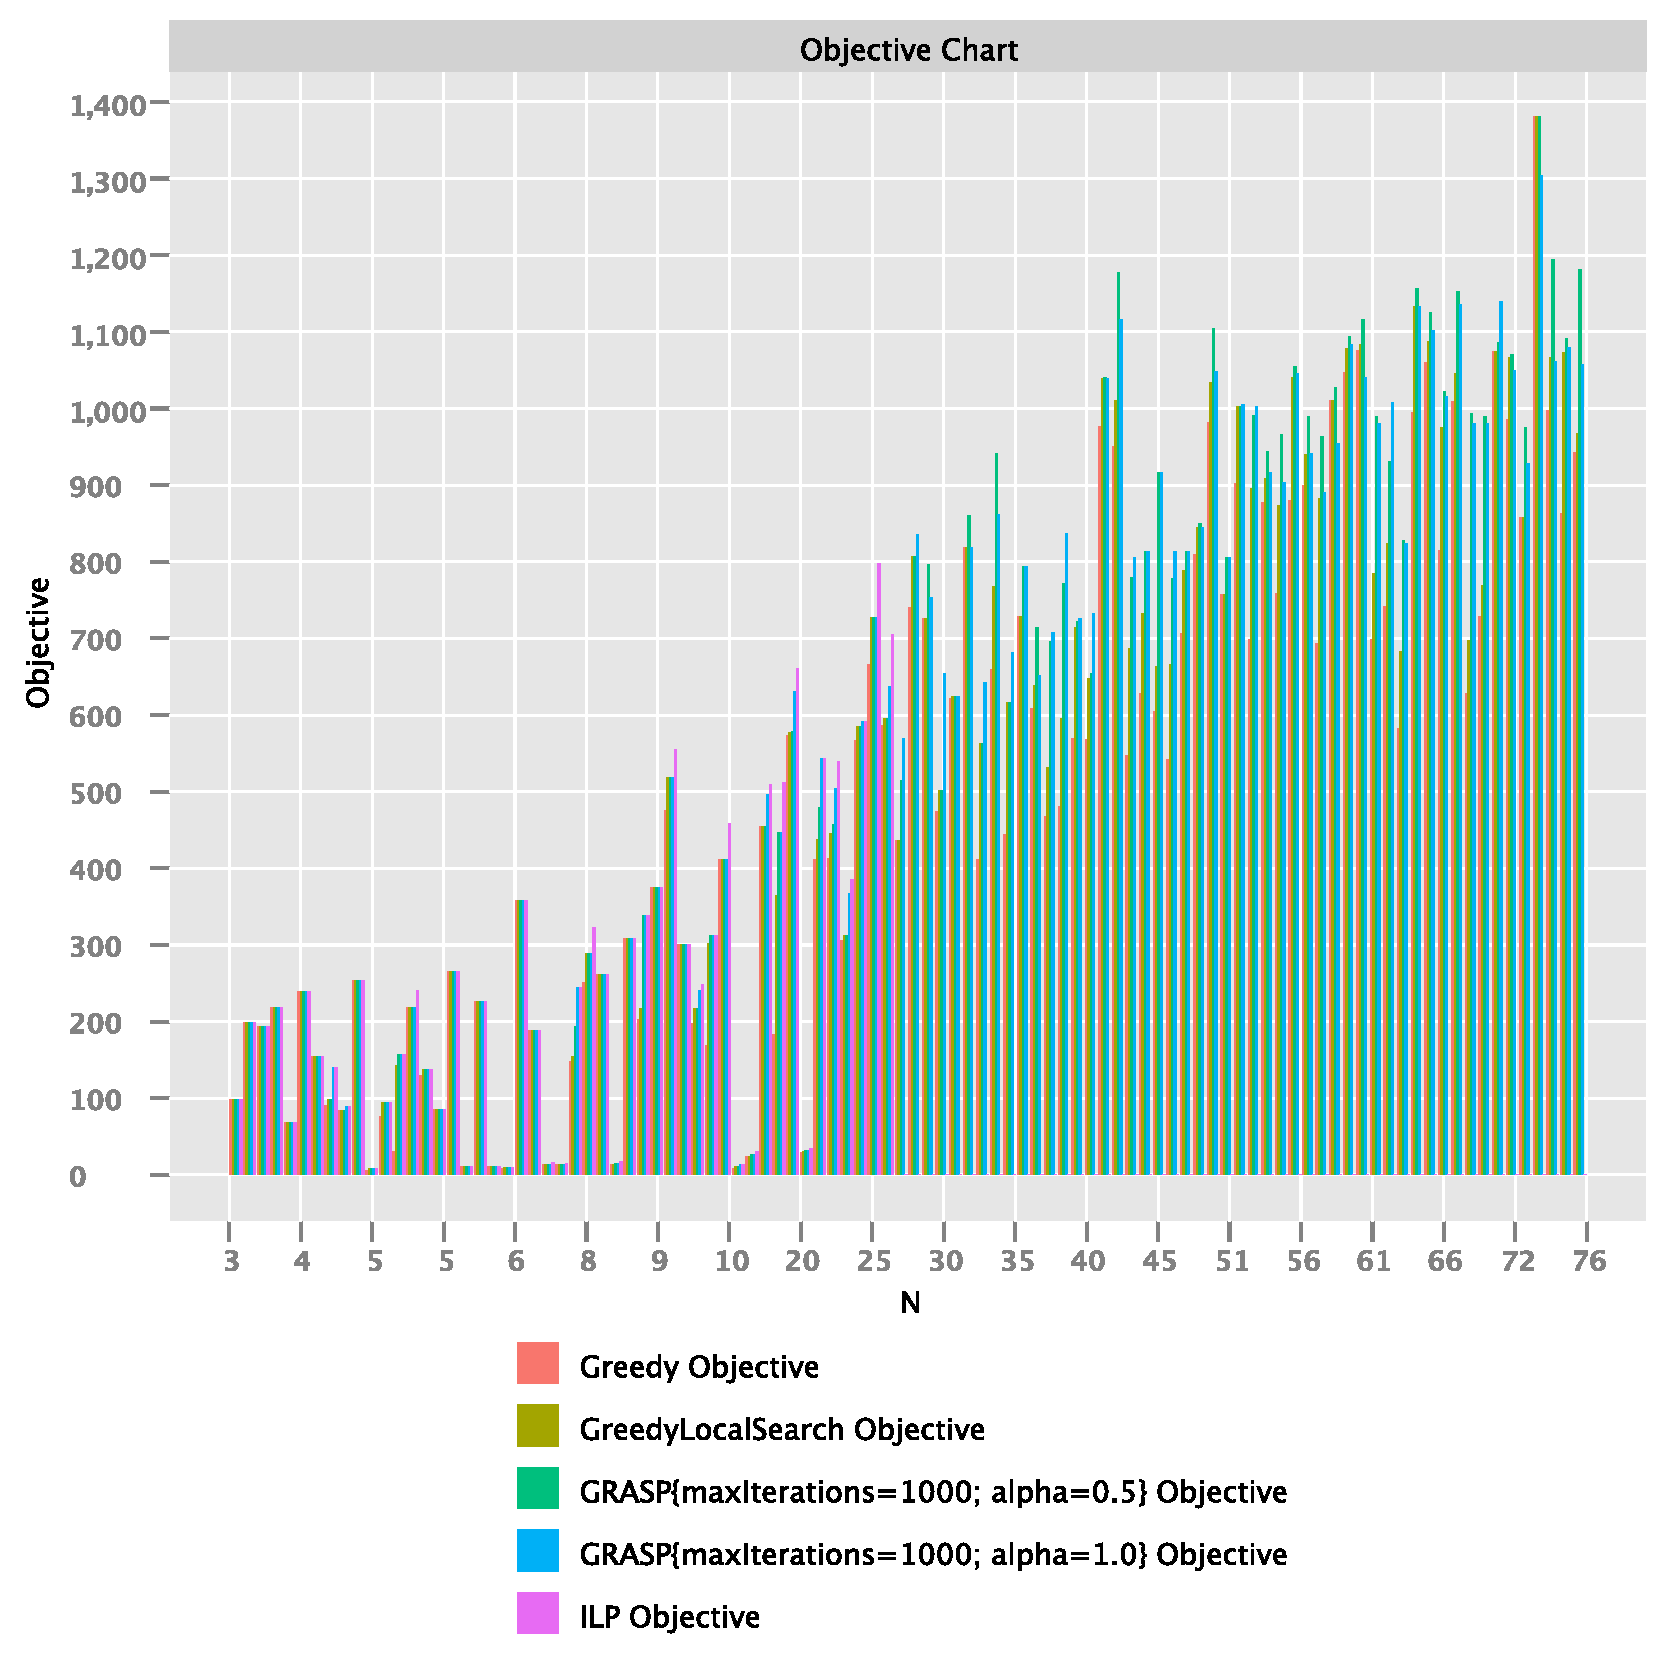
\includegraphics[width=0.8\textwidth]{./documentation/assets/objectiveChart.pdf}
\end{frame}

\end{document}